\clearpage
\twocolumn[{%
\rqparent
\subsection{Agreement with DataDecide}
\label{app:rq07_external_frameworks}

\noindent\begin{minipage}[t]{0.485\textwidth}
\vspace{0pt}
\paragraph{Research Question.} \emph{Do the SNR variants and the ``reliable benchmark'' set that we find on our ladder also hold on AllenAI's DataDecide / OLMo corpus, for the English benchmarks that both evaluate?}

\paragraph{Setup.} We test whether our ladder and DataDecide agree on which English tasks separate their models, using the SNR of each task on both. We compare our 1B rung (seed 1904, every cell, ladder and data build) with the 1B rung of DataDecide (25 data recipes). The tasks are the English tasks that both evaluate and that clear the above-chance gate on our side. SNR is the relative standard deviation of the final scores across models divided by the relative checkpoint noise (the \texttt{rel\_std} variant). We compare it on a log scale.
\end{minipage}\hfill
\begin{minipage}[t]{0.485\textwidth}
\vspace{0pt}
\begin{rqfinding}
\textbf{1. Both corpora rank the nine gated shared tasks in a similar order.} The Spearman $\rho$ is 0.77 and the Pearson r of log$_{10}$ SNR 0.77 (p = 0.016). With nine points, this is indicative, not robust. (Figure~\ref{fig:app_rq07_external_frameworks}.)
\\
\\
\textbf{2. Both corpora put BoolQ last and OpenBookQA near the bottom, but their top task differs (n = 9).} The \texttt{rel\_std} SNR is 4.09 / 8.18 / 2.97 / 4.94 / 2.64 / 1.78 / 3.51 / 3.23 / 1.35 on our ladder and 15.67 / 15.34 / 12.61 / 13.30 / 9.29 / 4.09 / 6.53 / 4.00 / 3.56 on DataDecide, for ARC Easy / HellaSwag / ARC Challenge / MMLU / CSQA / OpenBookQA / PIQA / Winogrande / BoolQ.
\\
\\
\textbf{3. Our SNR is 1.2--4.2$\times$ smaller.} DataDecide's \texttt{rel\_std} SNR exceeds ours by 4.2$\times$ on ARC Challenge, 3.8$\times$ on ARC Easy, 3.5$\times$ on CSQA, 2.7$\times$ on MMLU, 2.6$\times$ on BoolQ, 2.3$\times$ on OpenBookQA, 1.9$\times$ on HellaSwag, 1.9$\times$ on PIQA and 1.2$\times$ on Winogrande.
\end{rqfinding}
\end{minipage}

\vspace{\baselineskip}
\noindent\begin{minipage}{\textwidth}
\centering
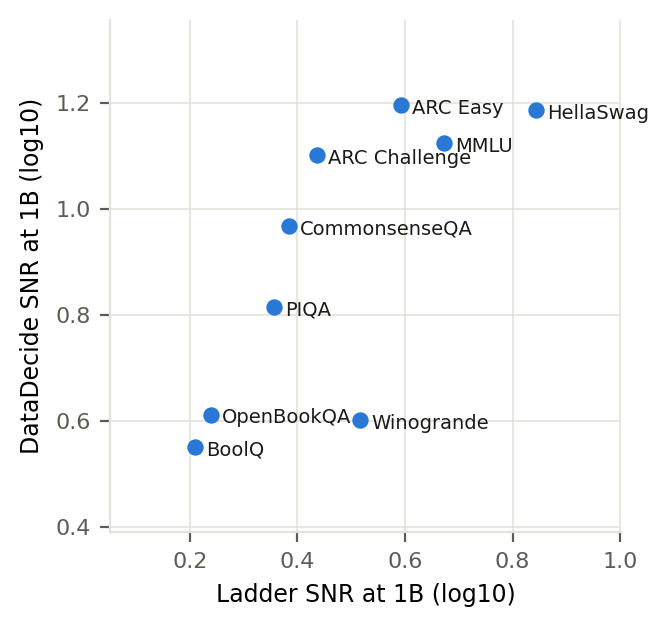
\includegraphics[width=\textwidth,height=0.36\textheight,keepaspectratio]{figures/app_rq07_external_frameworks.png}
% source: src/signal-and-noise/analysis/rq07_external_frameworks/pretraining/predictivity/snr_apertus_vs_snr_allenai_paper.png
\captionof{figure}{\textbf{Both corpora rank the nine gated shared tasks in a similar order.} Each point is one English task that both our ladder and DataDecide evaluate and that clears the above-chance gate on our side. The x axis gives the SNR of our 1B rung and the y axis the SNR of the DataDecide 1B rung, both on a log10 scale.}
\label{fig:app_rq07_external_frameworks}
\end{minipage}
}]
